\documentclass[10pt]{article}
\usepackage{../_macrosLatex/macros}
\usepackage[a4paper,margin=2.5cm]{geometry}
\usepackage{fancyhdr} % Gestion header/footer

%----------------------------------------------------
% Paramétrage de la fiche
%----------------------------------------------------
\matiere{BTS SNIR TS1}
\sequence{Programmation en langage C++}
\seqlogo{\faCode}
\titrefiche{C02 - Structures alternatives et répétitives}
\version{v1.0}
\dateversion{02.10.22}
\type{cours}

%----------------------------------------------------
% Définition des pieds et têtes de page
%----------------------------------------------------
% Pour toutes les pages
\pagestyle{fancy}
\fancyhead[L]{\seqlogo\ \sequenceVal}
\fancyhead[R]{\titreficheVal}
\fancyfoot[L]{\matiereVal - Lycée Louis Rascol, Albi}
\fancyfoot[R]{\ccbyncsaeu}
\fancyfoot[C]{\thepage\ / \pageref{LastPage}}
% Pour la première page
\fancypagestyle{firstpage}{%
    \lhead{}
    \rhead{}
    \renewcommand{\headrulewidth}{0pt}
}

%----------------------------------------------------
% Début du document
%----------------------------------------------------
\begin{document}
\cartouche
\thispagestyle{firstpage}

\introduction{assets/aiguillage.jpg}{Photo par \href{https://unsplash.com/@causeimluap}{causeimluap} sur \href{https://unsplash.com/}{unsplash}}{
    Dans ce cours, nous expliquons comment gérer le flux d'exécution d'un programme, nous découvrirons les structures alternatives
    et répétitives. 
    
    \smallskip
    Ces structures vont nous permettre respectivement de créer des programmes pouvant prendre une décision et exécuter des instructions en boucle suivant une condition donnée.\\
    Ces structures disponibles dans la majorité des langages de programmation, sont indispensables à l'implémentation d'algorithmes des plus
    simples aux plus évolués.
}

\licence

\tableofcontents
\clearpage

%----------------------------------------------------
% Section 1
%----------------------------------------------------
\section{Les structures alternatives}
Les structures alternatives permettent d'exécuter un bloc de code dans certaines conditions et un autre bloc dans d'autres
conditions. Elles agissent comme un aiguilleur au niveau du flux d'exécution en le dirigeant dans telle ou telle direction
suivant la condition donnée.

%--------------------
% Structure if
%--------------------
\subsection{Structure Si : \mintinline{cpp}`if`}

\subsubsection{Définition d'une structure \mintinline{cpp}`if`}

\smallskip
Nous donnons ci-dessous la structure d'un \mintinline{cpp}`if`:

\begin{wrapfigure}[10]{l}{\textwidth/2}
    \centering
    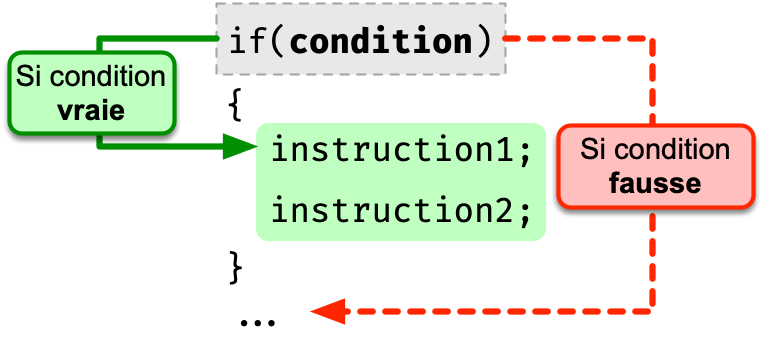
\includegraphics[max height=4cm,max width = \textwidth/2]{assets/if.jpg}
    \caption{Structure d'un \mintinline{cpp}`if`}
\end{wrapfigure}

Si la condition est \mintinline{cpp}`true` :
\begin{itemize}
    \item Les instructions présentes dans le corps du \mintinline{cpp}`if` sont \textbf{exécutées}.
    \item L'exécution continue sur la suite du code après le \mintinline{cpp}`if` 
\end{itemize}
Si la condition est \mintinline{cpp}`false` :
\begin{itemize}
    \item Les instructions présentes dans le corps du \mintinline{cpp}`if` sont \textbf{ignorées}
    \item L'exécution continue sur la suite du code après le \mintinline{cpp}`if` 
\end{itemize}

\smallskip
\subsubsection{Exemple 1 : Utilisation d'une structure \mintinline{cpp}`if`}
\begin{cppcode}
    #include <iostream>
    using namespace std;

    int main() {
        int nb;
        cout << "Entrez un entier : ";
        cin >> nb;

        if (nb > 0) {
            cout << "Vous avez entré un entier positif: " << number << endl;
        }

        cout << "Cette ligne est toujours exécutée.";

        return 0;
    }

\end{cppcode}
\captionof{listing}{Exemple 1 : Utilisation d'une structure \mintinline{cpp}`if`}

\bigskip
Sortie console pour une saisie utilisateur d'un entier positif : \mintinline{cpp}`42`  :

\begin{textcode}
    Entrez un entier : 42
    Vous avez entré un entier positif : 42
    Cette ligne est toujours exécutée.
\end{textcode}

Sortie console pour une saisie utilisateur d'un entier négatif : \mintinline{cpp}`-81`  :

\begin{textcode}
    Entrez un entier : -81
    Cette ligne est toujours exécutée.
\end{textcode}

Explications :

\begin{enumerate}
    \item Dans un premier temps nous déclarons \mintinline{cpp}`nb`, variable qui va recevoir le nombre entier saisi par l'utilisateur.
    \item Nous mettons ensuite une structure \mintinline{cpp}`if` dans laquelle la condition est sur l'entier \mintinline{cpp}`nb` : \mintinline{cpp}`nb > 0` 
    \item Si \mintinline{cpp}`nb` est strictement positif l'exécution sera aiguillée vers :\\
     \mintinline{cpp}`cout << "Vous avez entré un entier positif : " << number << endl;`
    \item Si \mintinline{cpp}`nb` est négatif ou égal à 0 l'exécution sera aiguillée hors de la structure \mintinline{cpp}`if` vers l'instruction suivante :\\
    \mintinline{cpp}`cout << "Cette ligne est toujours exécutée.";` 
\end{enumerate}

%--------------------
% Structure if...else
%--------------------
\subsection{Structure Si Sinon : \mintinline{cpp}`if ... else`}

\subsubsection{Définition d'une structure \mintinline{cpp}`if`}

\smallskip
Nous donnons ci-dessous la structure d'un \mintinline{cpp}`if`:

\begin{multicols}{2}
\begin{figure}[H]
    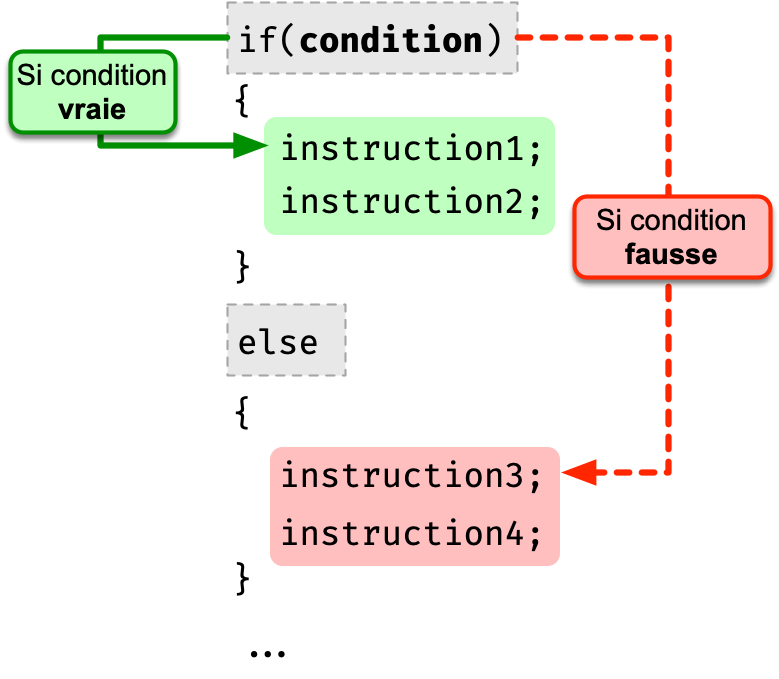
\includegraphics[max height=10cm,max width = \textwidth/2]{assets/ifElse.jpg}
    \centering
    \caption{Structure d'un \mintinline{cpp}`if...else`}
\end{figure}

Si la condition est \mintinline{cpp}`true` :
\begin{itemize}
    \item Les instructions présentes dans le corps du \mintinline{cpp}`if` sont \textbf{exécutées}.
    \item L'exécution continue sur la suite du code après le \mintinline{cpp}`if`
\end{itemize}
Si la condition est \mintinline{cpp}`false` :
\begin{itemize}
    \item Les instructions présentes dans le corps du \mintinline{cpp}`else` sont \textbf{exécutées}
    \item L'exécution continue sur la suite du code après le \mintinline{cpp}`if` 
\end{itemize}
\end{multicols}

\subsubsection{Exemple 2 : Utilisation d'une structure \mintinline{cpp}`if...else`}
\begin{cppcode}
    #include <iostream>
    using namespace std;

    int main() {
        int nb;
        cout << "Entrez un entier : ";
        cin >> nb;

        if (nb >= 0) {
            cout << "Vous avez entré un entier positif: " << number << endl;
        }
        else {
            cout << "Vous avez entré un entier négatif: " << number << endl;
        }

        cout << "Cette ligne est toujours exécutée.";

        return 0;
    }

\end{cppcode}
\captionof{listing}{Exemple 2 : Utilisation d'une structure \mintinline{cpp}`if...else`}

\bigskip
Sortie console pour une saisie utilisateur d'un entier positif : \mintinline{cpp}`42`  :

\begin{textcode}
    Entrez un entier : 42
    Vous avez entré un entier positif : 42
    Cette ligne est toujours exécutée.
\end{textcode}

Sortie console pour une saisie utilisateur d'un entier négatif : \mintinline{cpp}`-81`  :

\begin{textcode}
    Entrez un entier : -81
    Vous avez entré un entier négatif : -81
    Cette ligne est toujours exécutée.
\end{textcode}

Explications :

\begin{enumerate}
    \item Dans un premier temps nous déclarons \mintinline{cpp}`nb`, variable qui va recevoir le nombre entier saisi par l'utilisateur.
    \item Nous mettons ensuite une structure \mintinline{cpp}`if` dans laquelle la condition est sur l'entier \mintinline{cpp}`nb` : \mintinline{cpp}`nb >= 0` 
    \item Si \mintinline{cpp}`nb` est positif ou égal à 0 l'exécution sera aiguillée vers :\\
     \mintinline{cpp}`cout << "Vous avez entré un entier positif : " << number << endl;`
    \item Sinon l'exécution sera aiguillée vers : \\
    \mintinline{cpp}`cout << "Vous avez entré un entier négatif: " << number << endl;` 
    \item Une fois sorti de la structure \mintinline{cpp}`if` l'exécution du code continue et va sur l'instruction :\\
     \mintinline{cpp}`cout << "Cette ligne est toujours exécutée.";` 
\end{enumerate}

%----------------------
% Structure if..else if
%----------------------
\subsection{Structures Si imbriquées : \mintinline{cpp}`if ... else if`}


%------------------------
% Structure switch...case
%------------------------
\subsection{Structure Choix : \mintinline{cpp}`switch ... case`}



%----------------------------------------------------
% Section 2
%----------------------------------------------------
\section{Les structures répétitives}
\subsection{Boucle Tant que : \mintinline{cpp}`while()`}
\subsection{Boucle Faire Tant que : \mintinline{cpp}`do ... while()`}
\subsection{Boucle Pour : \mintinline{cpp}`for()`}


\end{document}  